\documentclass[a4paper]{article}
\usepackage{mathtext}
\usepackage[russian]{babel}
\usepackage{indentfirst}
\usepackage[pdftex]{graphicx}
\usepackage{multirow}
\usepackage{csvsimple}
\usepackage{amssymb}
\usepackage[left=2cm,right=2cm,top=2cm,bottom=2cm]{geometry}
% Название работы здесь
\def \work {Работа 2.1.3 Определение показателя адиабаты по скорости звука в газе}
\usepackage{fancyhdr}
\pagestyle{fancy}
\fancyfoot{}
\fancyhead[RE, RO]{\thepage}
\fancyhead[LE, LO]{\work}
\title{\work}
\author{Иван Сладков}
\begin{document}
\maketitle
\section{Аннотация}
\thispagestyle{empty}
% Текст аннотации пиши здесь
В данной работе производится измерение частоты колебаний и длины волны при резонансе звуковых колебаний в газе, заполняющем трубу, а также определение показателя адиабаты с помощью уравнения состояния идеального газа.
\section{Теоретические сведения}
% Теоретические сведения
Скорость распространения звуковой волны в газах зависит от показателя адиабаты $\gamma$. Скорость звука в газах определяется формулой
\begin{equation}
c = \sqrt{\gamma \frac{R T}{\mu}}.
\label{eq:СкоростьЗвука}
\end{equation}

Преобразуя эту формулу найдём
\begin{equation}
\gamma = \frac{\mu}{R T} c^2.
\label{eq:гамма}
\end{equation}
Таким образом, для определения показателя адиабаты достаточно измерить температуру газа и скорость распространения звука (молярная масса газа предполагается известной).

Если длина трубы равна целому числу полуволн, то
\begin{equation}
L = n \lambda / 2,
\label{eq:ДлинаВолны}
\end{equation}
где $L$ --- длина трубы, $\lambda$ --- длина волны, и $n \in \mathbb{N}$.

В данном опыте длина трубы постоянна, поэтому для последовательных резонансов применимы следующие формулы:
\begin{eqnarray}
\label{eq:ДлинаДляПосл}
L = \frac{\lambda_{k+1}}{2} (n + k) \\
f_{k+1} = f_1 + \frac{c}{2 L} k
\label{eq:Частота}
\end{eqnarray}
\section{Оборудование и инструментальные погрешности}
% Оборудование и инструментальные погрешности
Установка, использованная в данном опыте, изображена на рисунке \ref{fig:Установка}.
\begin{figure}[p]
	\centering
		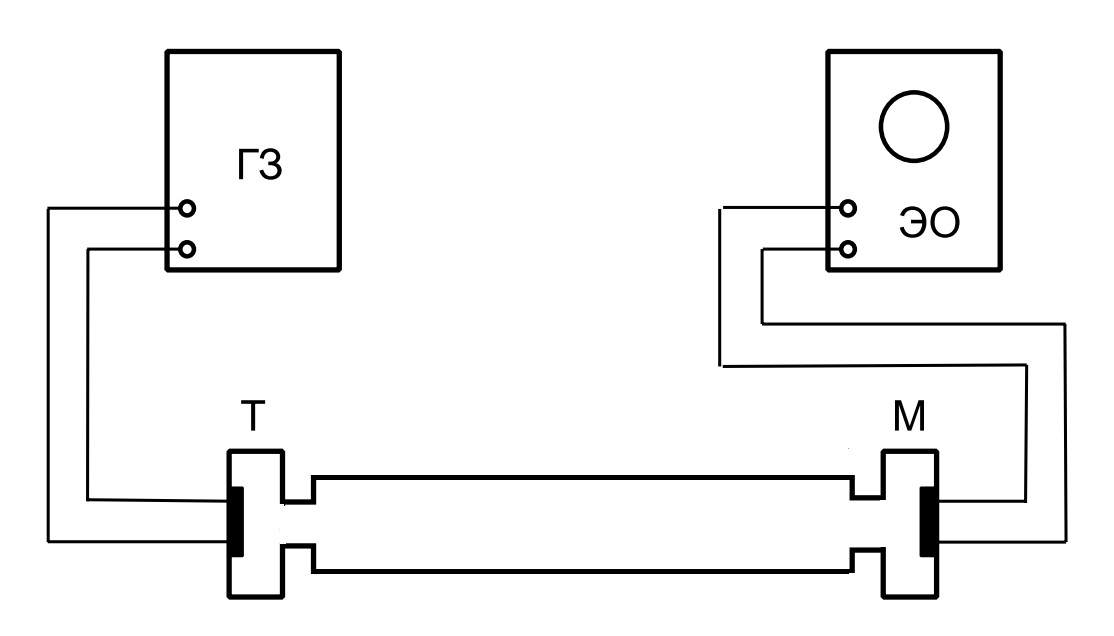
\includegraphics[width=1.00\textwidth]{1.jpg}
	\caption{Установка для определения показателя адиабаты}
	\label{fig:Установка}
\end{figure}
Для определения показателя адиабаты $\gamma$ применялась установка с нерегулируемой длиной трубы. В ходе опыта, с помощью звукового генератора (ГЗ) регулировалась частота производимого звука с целью получения резонанса.

{\bf Длина трубы: } $l = 79.5 \pm 0.5 $ см

{\bf Температура газов: } $T = 297.6 \pm 0.1 $ К

{\bf Погр. звукового генератора: } $\Delta = \pm 10 $ Гц

\section{Результаты измерений и обработка данных}
Результаты измерений представим в виде таблицы \ref{tab:РезультатыИзмерений}. 
\begin{table}[h]
	\centering
		\begin{tabular}{|l|l|l|l|l|l|l|l|l|l|l|l|}
\hline
$n$                    & \textbf{1} & \textbf{2} & \textbf{3} & \textbf{4} & \textbf{5} & \textbf{6} & \textbf{7} & \textbf{8} & \textbf{9} & \textbf{10} & \textbf{11} \\ \hline
$\nu({\rm O_2})$, Гц   & 220        & 586        & 655        & 867        & 1082       & 1284       & 1506       & 1718       & 1928       & ---         & 2361        \\ \hline
$\nu({\rm C O_2})$, Гц & 175        & 380        & 510        & 645        & 834        & 1002       & 1175       & 1338       & 1510       & 1676        & 1830        \\ \hline
\end{tabular}
	\caption{Результаты измерений}
	\label{tab:РезультатыИзмерений}
\end{table}
Проверена повторяемость результатов при возрастании и убывании частот. 10-й резонанс при измерениях для воздуха получить не удалось. Это может быть связано с высокой чувствительностью ручки <<Частота>> звукового генератора.

Построим график \ref{fig:Разность}, отображающий зависимость между $k$ и $f_{k+1}-f_1$.
\begin{figure}[p]
	\centering
		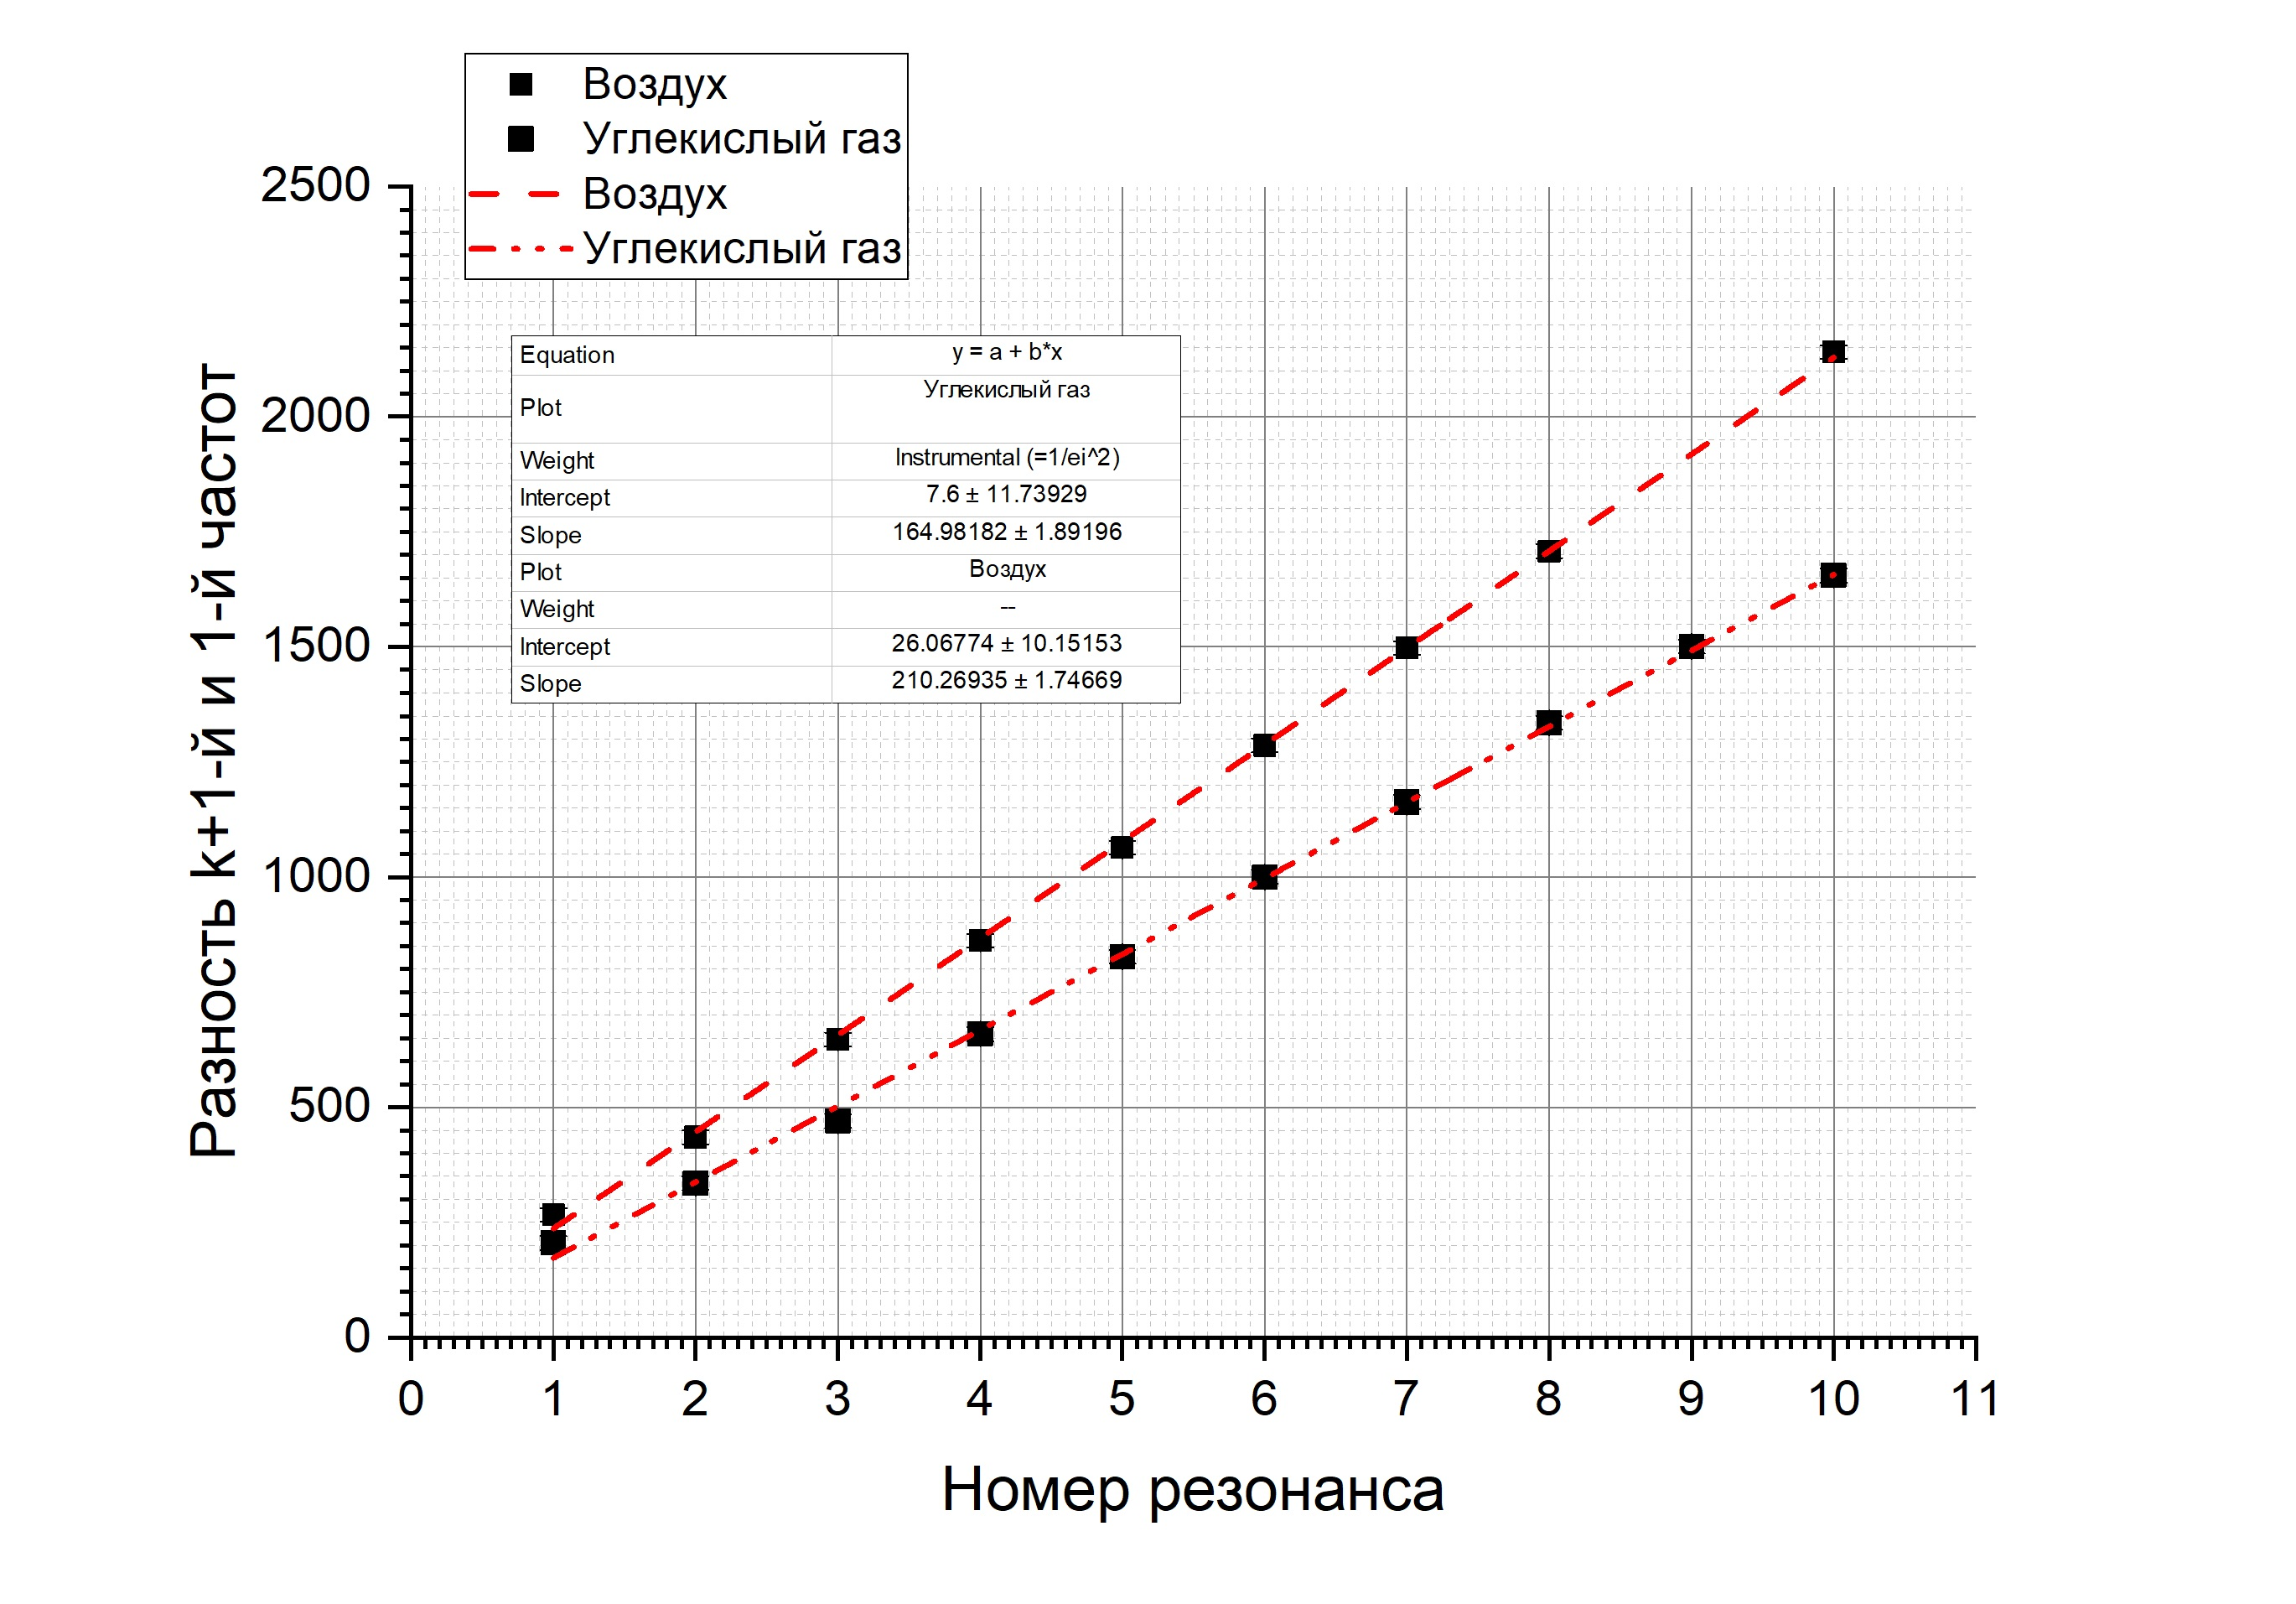
\includegraphics[width=1.00\textwidth]{2.jpg}
	\caption{Зависимость разности частот от номера резонанса}
	\label{fig:Разность}
\end{figure}
В таком графике, согласно формуле (\ref{eq:Частота}), угловой коэффициент равен $\frac{c}{2 L}$, откуда получим скорость звука: $c = 2 L k$, зная её, можем определить показатель адиабаты из формулы (\ref{eq:гамма}); посчитаем погрешности. Занесём результаты в таблицу \ref{tab:РасчётПоказателяАдиабаты}.

\begin{table}[h]
	\centering
\begin{tabular}{|l|l|l|l|l|}
\hline
                     & \textbf{k}  & \textbf{Скорость звука, см/с} & \textbf{Молярная масса, г/моль} & \textbf{Показатель адиабаты} \\ \hline
\textbf{Воздух}      & $210 \pm 2$ & $33430 \pm 350$               & 29                              & $1.30 \pm 0.03$              \\ \hline
{$\bf \rm C O_2$} & $165 \pm 2$ & $26230 \pm 340$               & 48                              & $1.33 \pm 0.03$              \\ \hline
\end{tabular}
	\caption{Расчёт показателя адиабаты}
	\label{tab:РасчётПоказателяАдиабаты}
\end{table}

\section{Вывод}
Произвели измерение частоты колебаний и длины волны при резонансе звуковых колебаний в газе, заполняющем трубу при её постоянной длине. На основе этих данных расчитали скорости звука в воздухе и углекислом газе; они оказались близки к табличным значениям. Это говорит о неплохой точности метода. С помощью уравнения состояния идеального газа определили показатели адиабаты каждого газа.
\end{document}

